%
% 98-127
% Lecture 02: A First Look at Unity
% 
% Template adapted from
% https://www.cs.cmu.edu/~15150/previous-semesters/2012-spring/resources/latex/template.tex
%

\documentclass[11pt]{article}

\usepackage{amsmath}
\usepackage{amssymb}
\usepackage{amsthm}
\usepackage{hyperref}
\usepackage{fancyhdr}
\usepackage{listings}
\usepackage{color}
\usepackage{graphicx}
\usepackage{setspace}
\usepackage{times}
\usepackage{wrapfig}
\usepackage{fontawesome}

\usepackage{menukeys}

\oddsidemargin0cm
\topmargin-2cm
\textwidth16.5cm
\textheight23.5cm

\newtheorem{lemma}{Lemma}

%% Begin Constants %% <-- (edit these!)

% Lecture Info
\newcommand{\lecturenum}{2}
\newcommand{\lecturename}{A First Look at Unity}

% Author of THIS document
\newcommand{\authorname}{Adrian Biagioli}

% Course Info
\newcommand{\coursenum}{98-127}
\newcommand{\coursename}{Game Creation for People Who Want to Make Games}
\newcommand{\coursesem}{S20}

% Instructors of course
\newcommand{\instructors}{\begin{minipage}[t]{0.4\columnwidth}\centering Adrian Biagioli (\,\href{mailto:abiagiol@andrew.cmu.edu}{abiagiol@andrew.cmu.edu}\,) \\ Carter Williams (\,\href{mailto:ncwillia@andrew.cmu.edu}{ncwillia@andrew.cmu.edu}\,)\end{minipage}
\begin{minipage}[t]{0.4\columnwidth}\centering Woody McCoy (\,\href{mailto:mwmccoy@andrew.cmu.edu}{mwmccoy@andrew.cmu.edu}\,) \\ Sebastian Yang (\,\href{mailto:yukaiy@andrew.cmu.edu}{yukaiy@andrew.cmu.edu}\,)\end{minipage}}

% Math shortcuts
\newcommand{\work}{\mathcal{W}}
\newcommand{\expv}{\mathbf{E}}
\newcommand{\pr}{\mathbf{Pr}}
\newcommand{\ts}{\textsuperscript}
\newcommand{\bigo}{\mathit{O}}

%% End Constants %%

%% Begin syntax highlighting settings %%

\definecolor{dkgreen}{rgb}{0,0.6,0}
\definecolor{gray}{rgb}{0.5,0.5,0.5}
\definecolor{mauve}{rgb}{0.58,0,0.82}

\lstset{frame=tb,
    language=ML,
    aboveskip=3mm,
    belowskip=3mm,
    showstringspaces=false,
    columns=flexible,
    basicstyle={\small\ttfamily},
    numbers=left,
    stepnumber=1,
    numberstyle=\tiny\color{gray},
    keywordstyle=\color{blue},
    commentstyle=\color{dkgreen},
    stringstyle=\color{mauve},
    breaklines=true,
    breakatwhitespace=true,
    tabsize=3
  }

\lstnewenvironment{pseudocode}[1][]
{
    \lstset{
        mathescape=true,
        frame=tb,
        numbers=left, 
        basicstyle=\small, 
        numberstyle=\tiny\color{gray},
        keywordstyle=\color{black}\bfseries\em,
        commentstyle=\color{dkgreen},
        stringstyle=\color{mauve},
        keywords={,input, output, return, datatype, function, in, if, else, foreach, while, begin, end, }
        numbers=left,
        breaklines=true,
        breakatwhitespace=true,
        tabsize=3
    }
}
{}

% From https://tex.stackexchange.com/questions/95036/continue-line-numbers-in-listings-package
\def\ContinueLineNumber{\lstset{firstnumber=last}}
\def\StartLineAt#1{\lstset{firstnumber=#1}}
\let\numberLineAt\StartLineAt

%% End syntax highlighting settings %%

\setlength{\parindent}{2em}
\setlength{\parskip}{5pt plus 1pt}
\renewcommand{\baselinestretch}{1.15}

\pagestyle{fancyplain}
{
    \lhead{\fancyplain{}{Lecture \lecturenum}}
    \rhead{\fancyplain{}{\coursenum}}
    \chead{\fancyplain{}{\lecturename}}
}
\setlength{\headheight}{14pt}

\graphicspath{ {./images/} }

\begin{document}

\thispagestyle{plain}
{
    \vspace{1.5em}
    \begin{center}
    {
        \huge
        Lecture \lecturenum \\
        \vspace{0.5em}
        \lecturename
        \vspace{0.4em}
    } \\
    {
        \it
        \coursenum: \coursename\ \ (\coursesem)
    } \\
    \vspace{1.0em}
    Written by \authorname \\
    \vspace{0.7em}
    Instructors:\\ \instructors
    \end{center}
}

\section{Objectives}

By the end of this lesson you will be able to:
\begin{itemize}
    \item Understand what a Game Engine is, and why we use the Unity game engine
    \item Utilize common Unity editor functionality and navigate scenes
    \item Understand Unity's high level architecture: the Scene Graph and GameObjects
    \item Utilize the inspector to design levels, given art assets and scripts
\end{itemize}

\noindent These lecture notes were written for {\bf Unity 2019.2.3f1}.

\section{What is a Game Engine?}

\par Video Games are a very complicated technical challenge.  Think about all of the stuff that goes on in your average video game, like Call of Duty.  There is a complicated {\it Graphics Pipeline}, which is the code that communicates very quickly with the user's graphics processor to produce complicated effects (shadows, explosions, hair, muzzle flashes\dots the list goes on).  There is also usually a {\it Physics Engine} that attempts to simulate how objects would interact with each other (for example, it would figure out how a grenade bounced throughout the scene).  There's also some sort of {\it Audio Mixer} that handles audio effects (for example, a low-pass filter when you are hit with a flashbang).  Then there's the {\it Animation Engine}, which allows characters to move around the scene realistically.  Many games include {\it Artificial Intelligence}, {\it UI Systems}, and more.

\par That's a lot of things that {\it many} games have in common!  In fact, it seems like a waste of time to re-do all of these complicated systems for every game that we want to make.  This is why Game Engines exist.  A {\bf Game Engine} aims to simplify game development by doing all the hard stuff for us (i.e. everything I mentioned in the previous paragraph).  This allows game designers like ourselves to focus on the good stuff: how to make our game fun.  In addition to this, game engines also tend to simplify {\it how we code} our games.  Many ``game-engine-less'' games are simply written in C++, which can be hard for beginners.  In contrast, Unity is in C\#, which is much more approachable.


{\bf Unity} is the most popular Game Engine out there right now for indie game developers, and it is the one that we will use in this course.  Right now, Unity's biggest competitor is the {\bf Unreal Engine 4} (UE4), which is developed by Epic Games (creators of {\it Gears of War} and {\it Fortnite}).  UE4 rivals Unity in many respects and outshines it in some (many will argue that UE4 has better builtin graphics than Unity), but we will not use it in this class because it is generally harder to use for beginners and requires knowledge of C++.  Another important difference is how you need to pay royalties if you decide to sell your game: Unity allows you to sell your game without paying any royalties, {\it until} your game makes \$100k per year.  After that point, you need to upgrade to Unity \href{https://store.unity.com}{``Plus'' or ``Pro''}, which has a monthly fee.  Unreal requires a 5\% royalty of all revenue of your game past \$3000, but has no Plus or Pro tier.

\section{Getting Started with Unity}

If you haven't already, download Unity:
\begin{itemize}
\item You can download Unity at \href{https://store.unity.com/download}{https://store.unity.com/download}.  Accept the license terms and click ``Download Unity Hub''.  The {\bf Unity Hub} is an application that you can use to browse Unity projects and install new Unity versions.  To install a new Unity Version, navigate to \menu{Installs > Add} in the Unity Hub interface.
\item If you're a programmer running Windows or Mac, I would recommend downloading Microsoft Visual Studio.  Visual Studio and Visual Studio for Mac both have great integration with Unity and are better than the default MonoDevelop: \href{https://www.visualstudio.com}{https://www.visualstudio.com}.
\end{itemize}

\begin{wrapfigure}{r}[50pt]{0.5\textwidth}
    \centering
    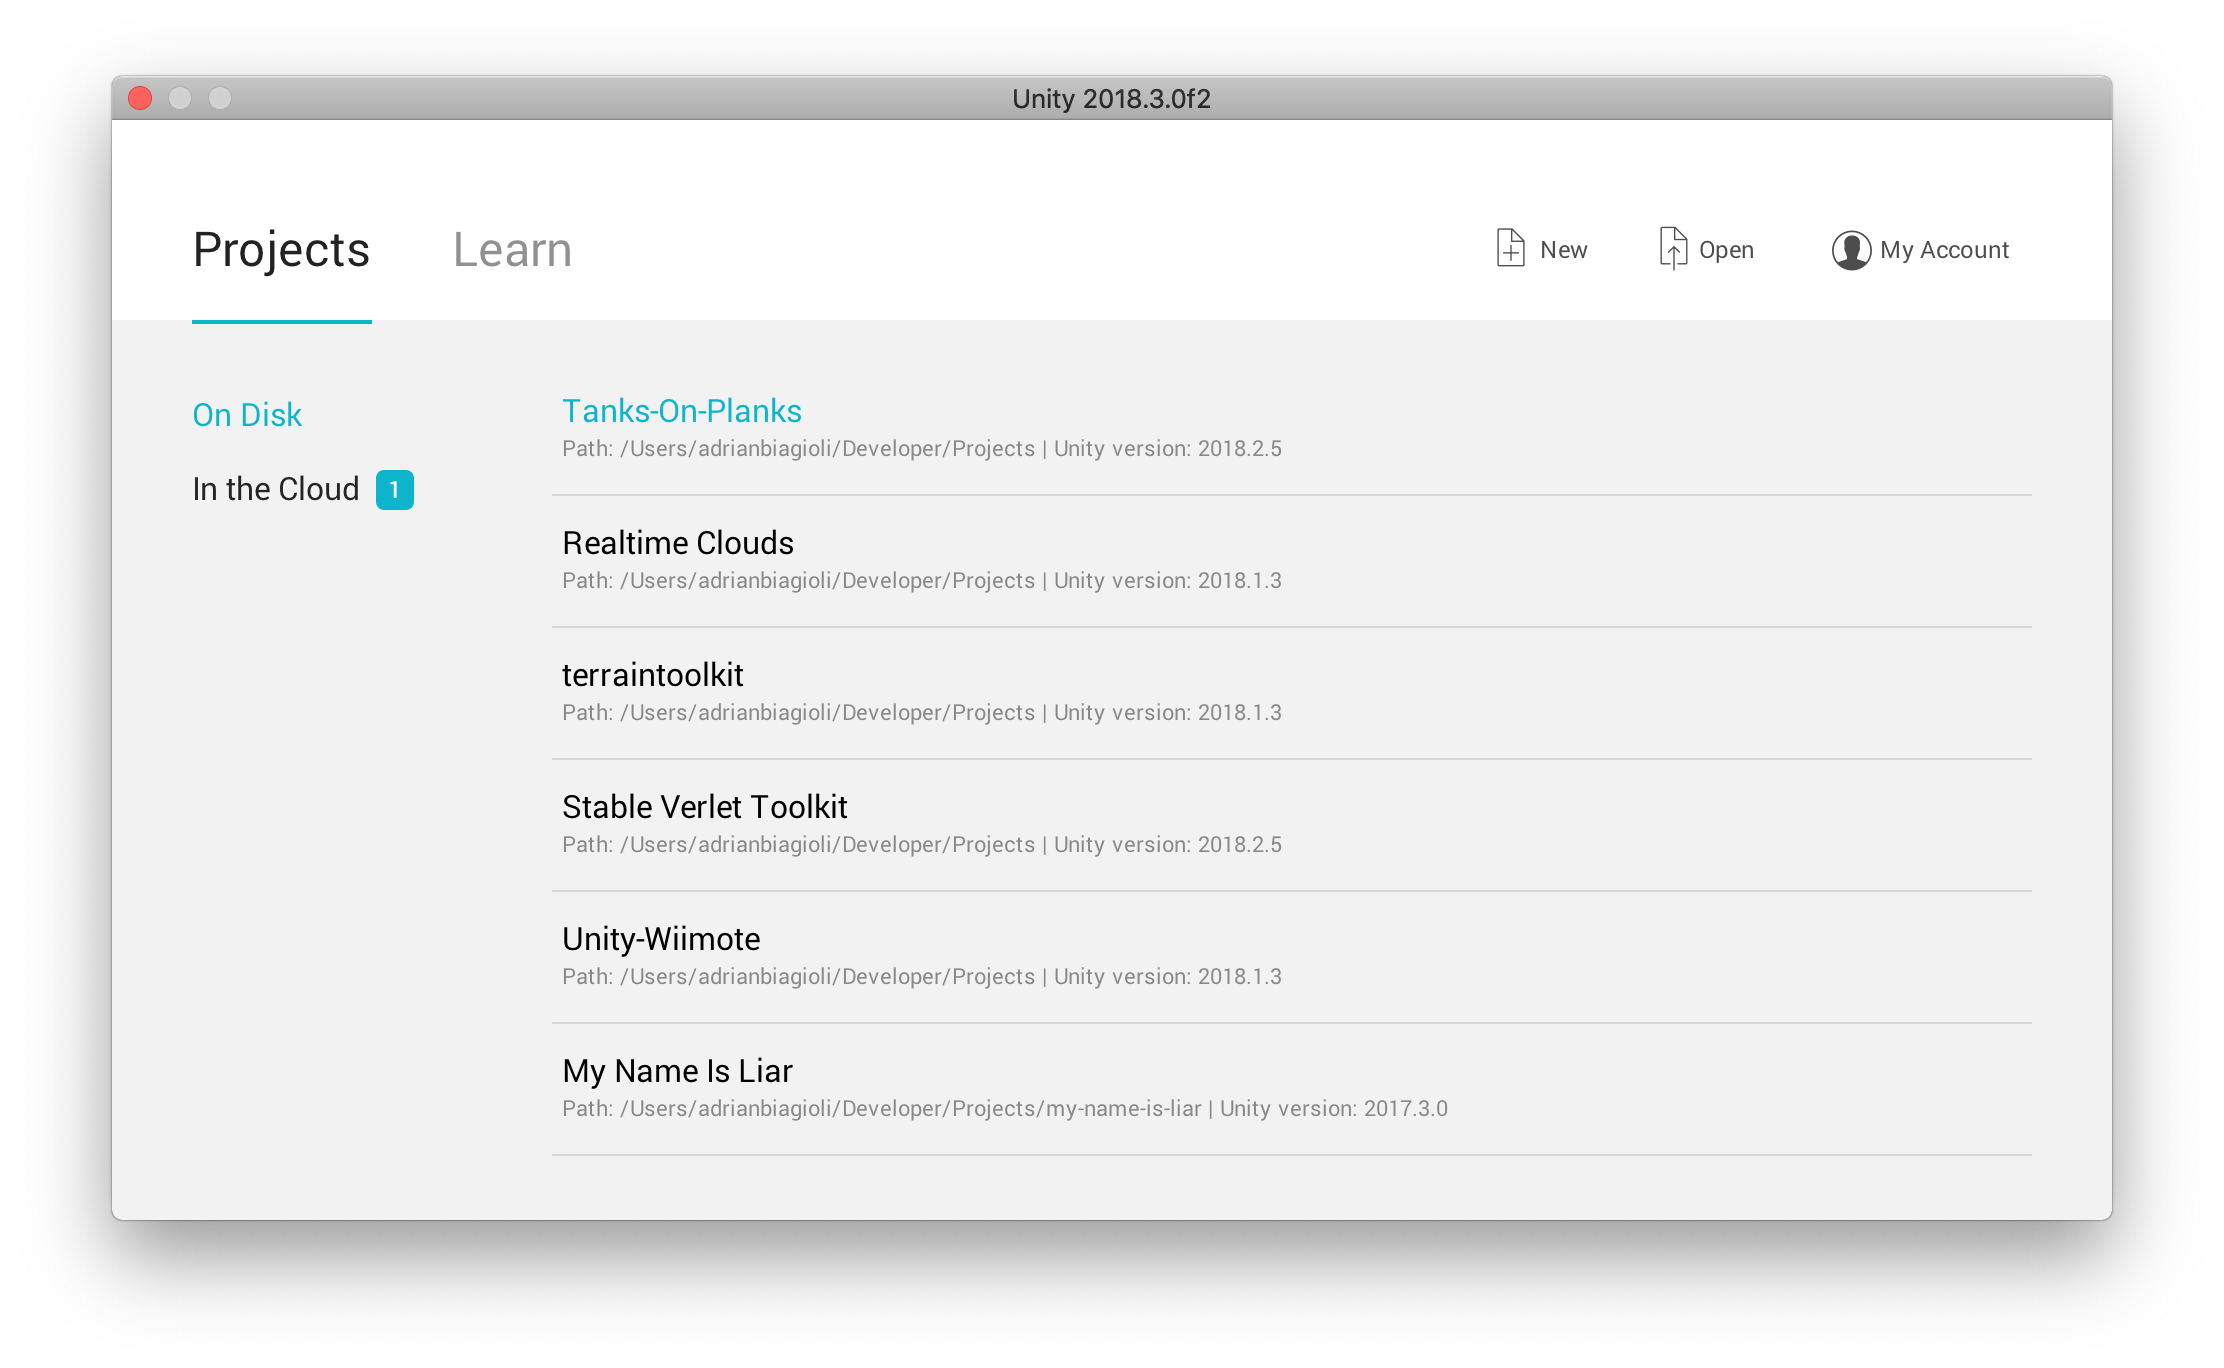
\includegraphics[width=0.5\textwidth]{proj-select}
    Unity Project Select Window
\end{wrapfigure}


When you open Unity Hub, you will first see the {\bf project selection screen}.  You may need to create a Unity account—do so if prompted.  Click ``new project'' on the top right of the window.

Enter a name for your new project (``Lecture 2 Project'') and specify a location for the project folder.  Make sure ``3D'' is checked.  Then click {\it create project}.  \textbf{Unity projects are saved in folders on your machine}, so if you browse to the project location you gave then you will find the Unity project files.

The Unity editor should now appear.  The editor is divided into \textbf{panels}, each providing a different way to interact with your Unity project.  If your editor doesn’t look like the one on the next page, click \menu{Layout > Default} on the top right of the editor.  Notice that panels can be reorganized and redocked to other panels by clicking and dragging on the tab at the top of each pane.  You can also resize panels and drag them out to their own window.

\pagebreak
\section{Basic Unity Editor Panels}

{
\centering \noindent
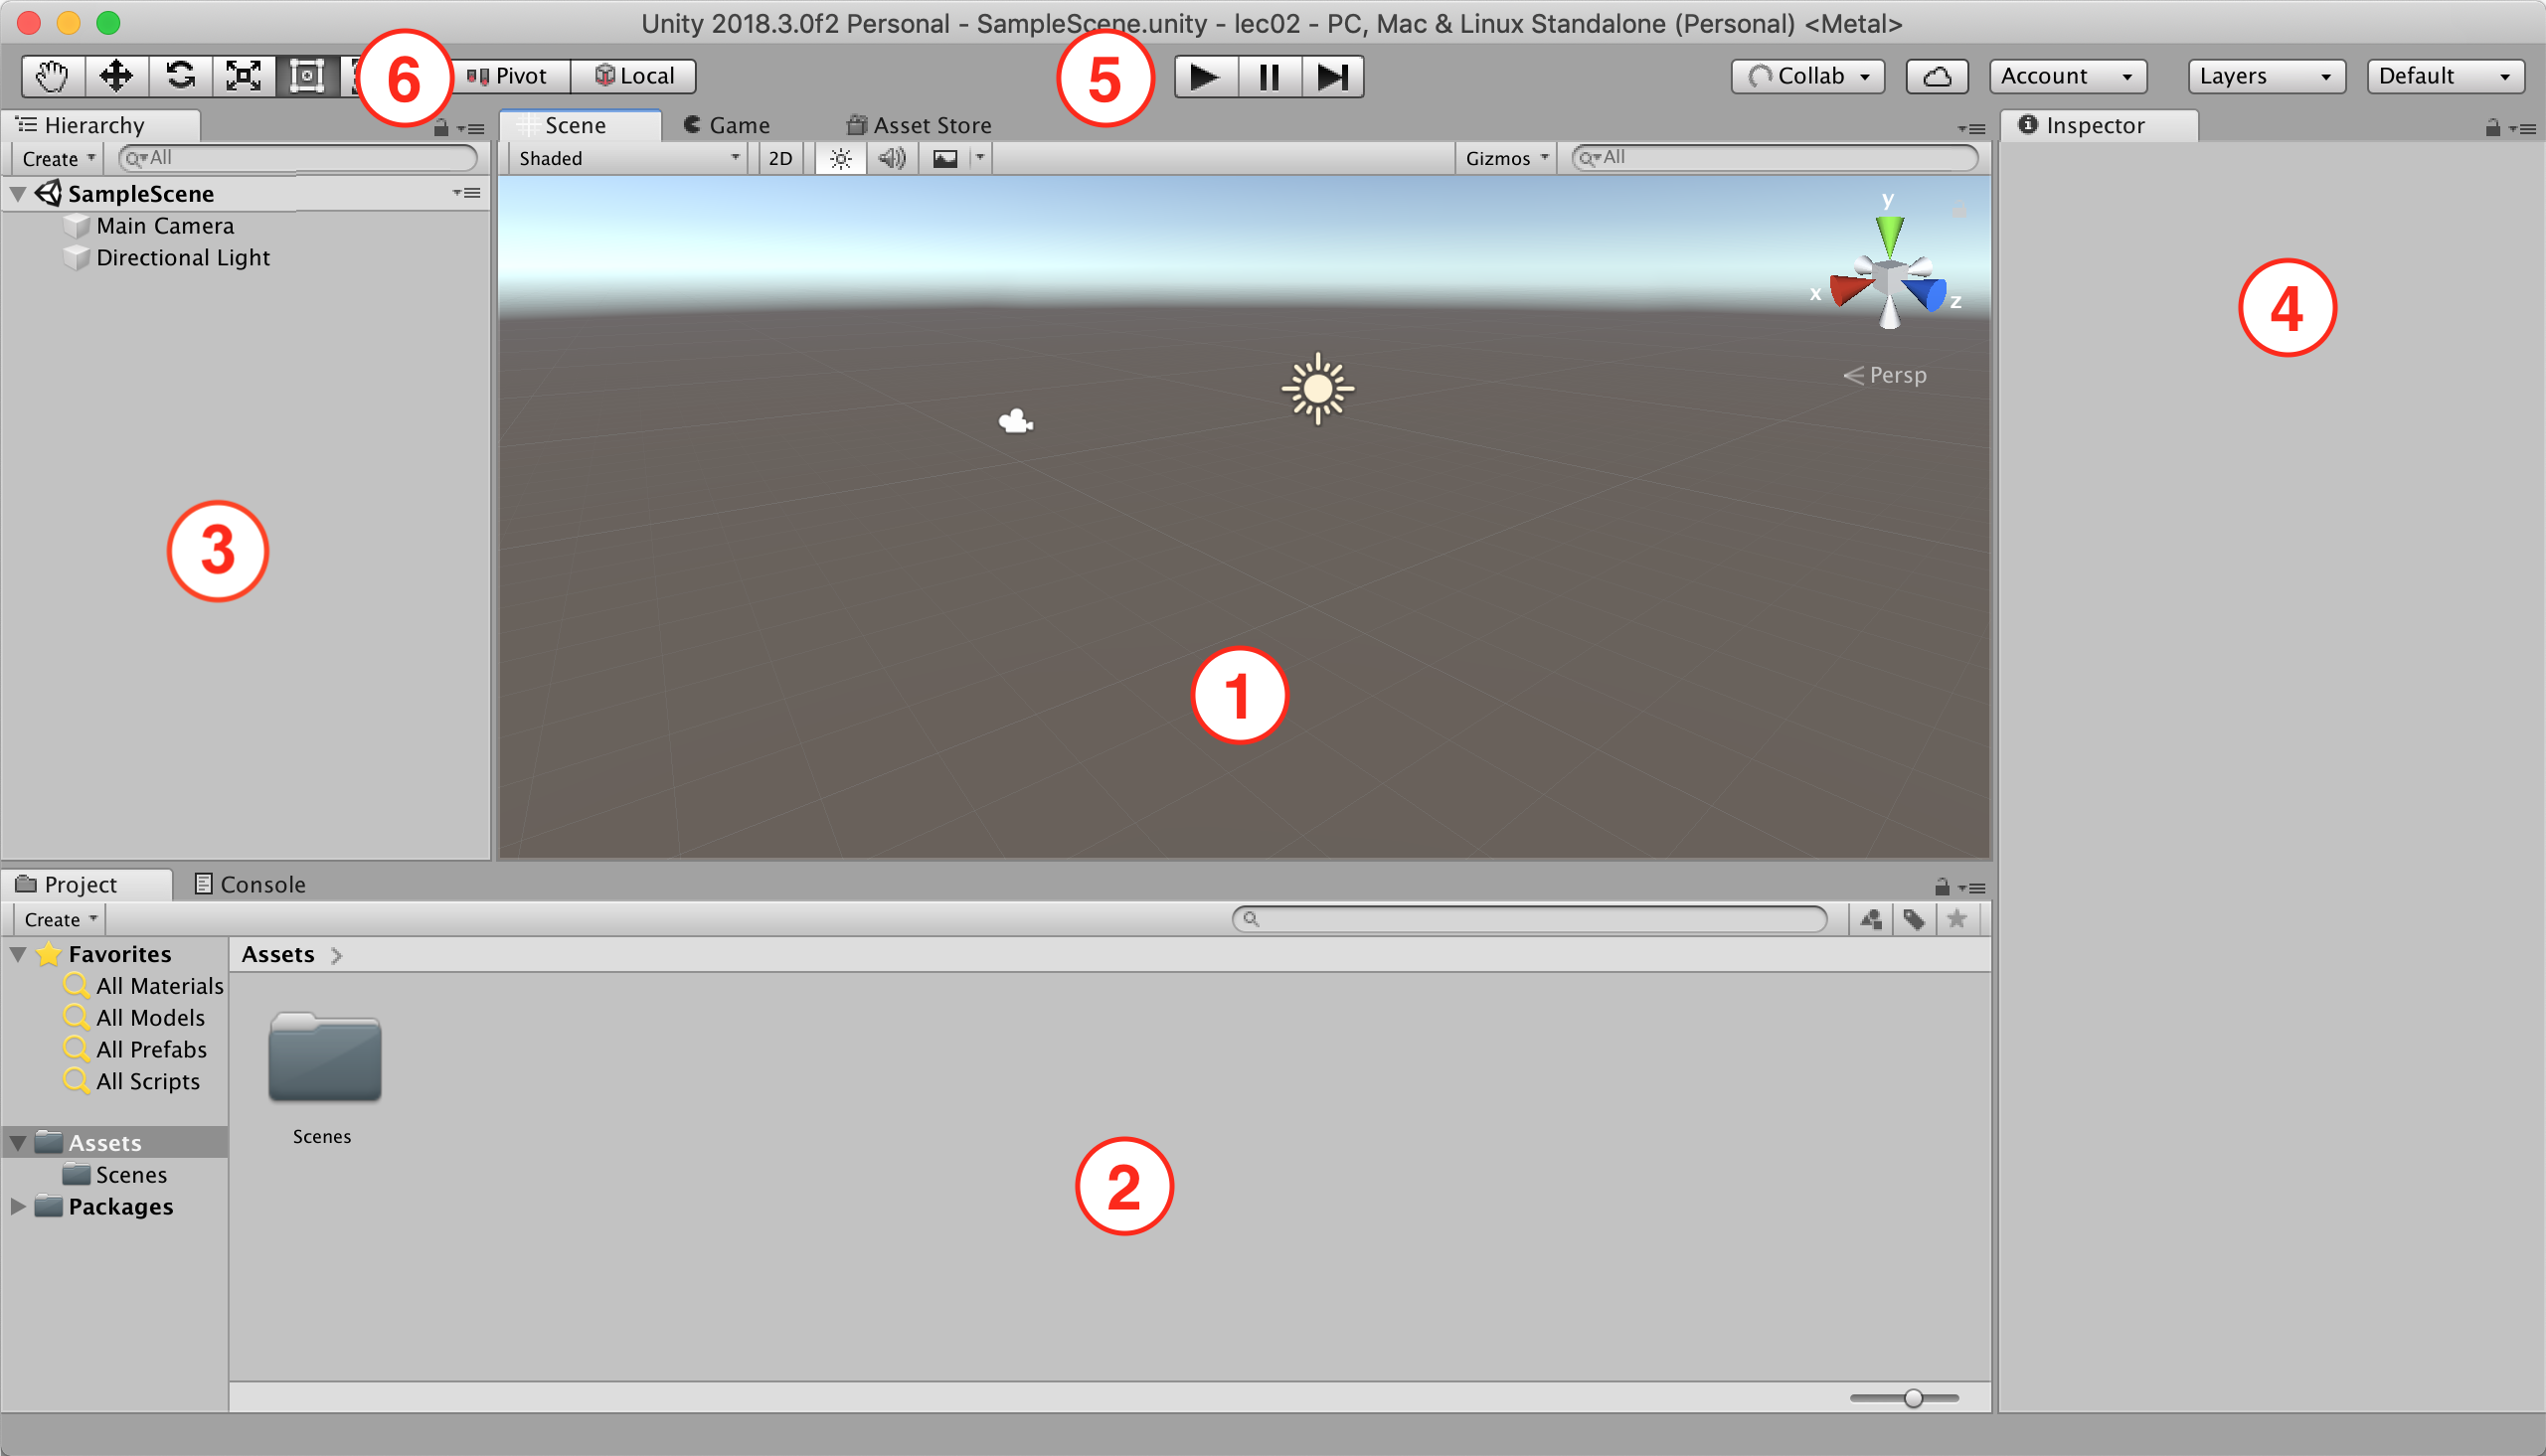
\includegraphics[width=1.0\textwidth]{basic-editor-panes}
}

This is the default configuration of the Unity editor, opening a freshly-made project.  Each panel that you see in the above screenshot is labeled as follows:

\begin{enumerate}
    \item The \textbf{Scene View} allows you to look into the game world from a perspective other than the in-game camera.  You can navigate the scene view as follows:
    \begin{itemize}
        \item \textbf{Right Click + Drag}: Look around
        \item \textbf{Right Click + WSADQE}: Move camera (FPS controls).  Hold shift to move faster.
        \item \textbf{Left Click}: Select and manipulate objects (see item 6 below)
    \end{itemize}
    \item The \textbf{Project Window} is a view into the assets of your game.  \textbf{Assets} are normal files that your game will use like scripts, 3D Models, textures (images), audio, animation data, scene files, and more.  The project window behaves much like the Finder on macOS or Explorer on Windows.
    \begin{itemize}
        \item In fact, these files are located in the \directory{/Assets} subfolder of your Unity project!  Try right clicking on a file in the project window and select ``Reveal\dots''
    \end{itemize}
    \item The \textbf{Hierarchy View} lists all of the \textbf{GameObjects} that are currently in the scene.
    \begin{itemize}
        \item In Unity terminology, a \textbf{GameObject} is any ``thing'' in your game.  \textit{Everything is a GameObject}: the player, a fence, an enemy, a weapon, a button, an NPC, a scoreboard, \dots.  Right now there are two GameObjects in the scene, a Main Camera and a Directional Light for the Sun.
        \item You can select a GameObject by clicking on it: either in the scene view or the hierarchy view.
        \item If you double click on a GameObject in the hierarchy view you can focus on it in the scene view.
    \end{itemize}
    \item The \textbf{Inspector} allows you to inspect and modify the properties of whichever GameObject or Asset is selected.  For example, you can change the position of a GameObject or the name of a file.  More information on how to use the Inspector will follow.
    \item The \textbf{Play Button} (\,\faPlay\,) will shift focus from the Scene View to the \textbf{Game View}, allowing you to play your game in real time!  When you are in ``Play Mode'', you can switch back to the Scene/Hierarchy/Inspector Panels and continue to modify the scene.  However, as soon as you stop playing (by clicking the play button again) \underline{your changes will revert to before you started playing}, so be careful!  While playing, you can also click the \textbf{Pause Button} (\,\faPause\,) to pause execution of the game (you can still make changes in the Scene View / Inspector while paused).  While paused, you can click the \textbf{Advance Frame Button} (\,\faFastForward\,) to advance by one frame.
    \item The \textbf{Scene View Tools} change the currently-active manipulator in the scene view.  These manipulators allow you to move, rotate, and scale GameObjects--more on this later.
\end{enumerate}

\section{The Scene Graph and GameObjects}

\begin{wrapfigure}[13]{r}[50pt]{0.45\textwidth}
    \centering
    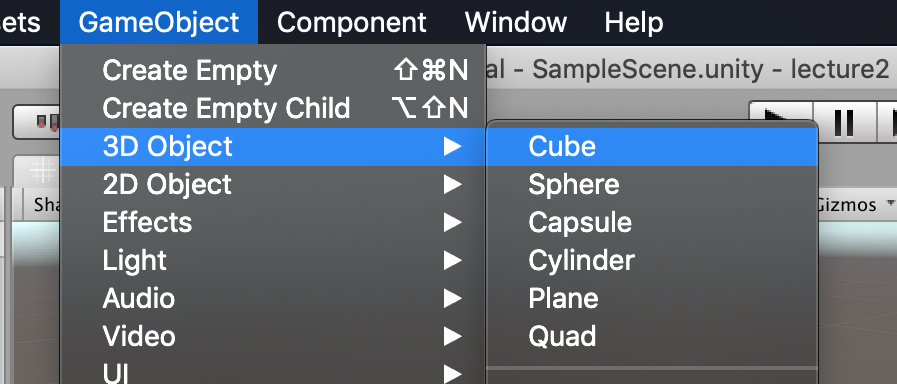
\includegraphics[width=0.45\textwidth]{cube-menu-item}\\
    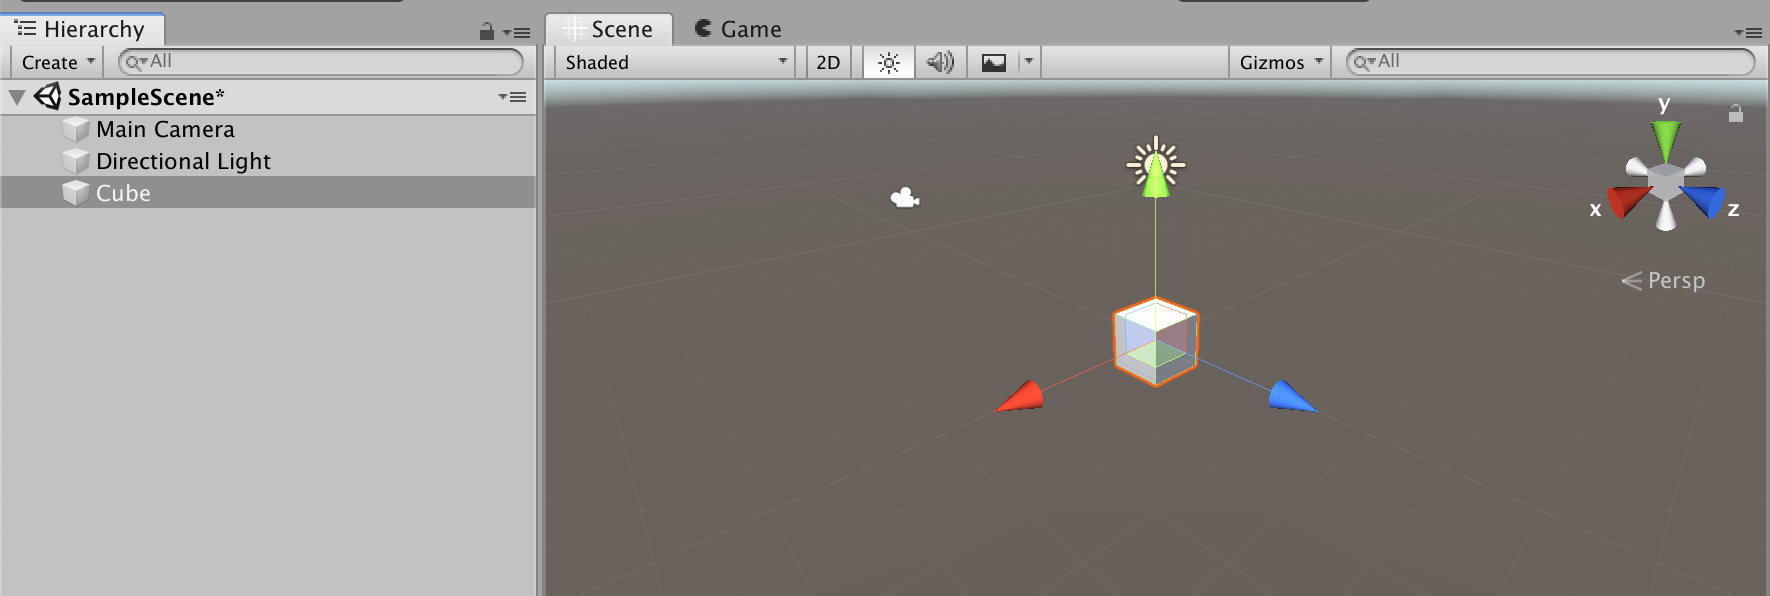
\includegraphics[width=0.45\textwidth]{newcube}
\end{wrapfigure}

When you first open Unity, the default scene (Called \texttt{SampleScene}) is loaded.  In Unity, a \textbf{Scene} can be considered a ``Level'' or a ``Screen'' in your game.  Scenes are saved to a .scene file in your Assets folder.  As mentioned above, there are two GameObjects currently in the scene: a Main Camera and an Directional Light.  If you don't see any GameObjects in the hierarchy view when you load the project, click on the small triangle next to \texttt{SampleScene} in the hierarchy view to expand it.  Let's add a third GameObject in the scene; navigate to \menu{GameObject > 3D Object > Cube} as shown on the right, and a cube should appear in your scene.  Notice the new entry ``Cube'' in the scene hierarchy view.

\subsection{Manipulating GameObjects with Scene View tools}

The Scene View Tools are located at the top left of the Unity window and are accessible at any time.  You can use the \keys{Q}\keys{W}\keys{E}\keys{R}\keys{T}\keys{Y} keys as a shortcut:

\begin{center}
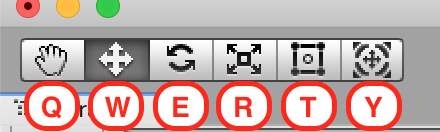
\includegraphics[width=0.5\textwidth]{scene-view-tools}
\end{center}

\noindent Here are each of the manipulators, from left to right:

\begin{enumerate}
    \item The \textbf{Pan Tool} 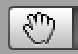
\includegraphics[width=20pt]{tool_pan.png} allows you to click and drag on the Scene View to pan the camera left / right / up / down relative to where you are looking.  You do not need to have the Pan Tool selected to right click + drag to move the camera, however.
    \item The \textbf{Move Tool} 
\includegraphics[width=20pt]{tool_move.png} shows a widget when selecting any GameObject that allows you to translate the GameObject throughout the world.  Try moving the cube that you made left and right inside the scene.  You can hold \keys{\cmd Cmd} on Mac or \keys{\ctrl} on Windows to snap GameObject translation to regular increments; navigate to \menu{Edit > Snap Settings\dots} to customize snapping settings.
    \item The \textbf{Rotate Tool} 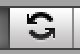
\includegraphics[width=20pt]{tool_rot.png} shows a similar widget that allows you to rotate GameObjects.  You can click and drag on the Red/Blue/Green circles to constrain rotation to one axis, or you can click and drag elsewhere on the widget to rotate the GameObject freely.  Again, you can hold \keys{\cmd Cmd} on Mac or \keys{\ctrl} on Windows to snap rotation to regular degree increments.  As with translation you can customize snapping via \menu{Edit > Snap Settings\dots}.
    \item The \textbf{Scale Tool} 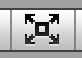
\includegraphics[width=20pt]{tool_scale.png} similarly allows you to scale objects in any dimension.  You can scale in all dimensions by clicking and dragging on the white box in the center of the widget.  Snapping can be used with the scale tool as well.
    \item The \textbf{Rect Tool} 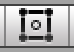
\includegraphics[width=20pt]{tool_rect.png} is generally used in place of the other transformation tools for 2D games and UI elements.  It allows you to easily move and scale rectangular objects in the X and Y dimensions.
    \item The \textbf{Transform Tool} 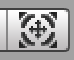
\includegraphics[width=20pt]{tool_trans.png}, added in a recent version of Unity, combines the Move / Rotate / Scale tools into one multi-purpose widget.
\end{enumerate}

\subsection{Parenting GameObjects}

Two GameObjects can also be \textbf{Parented} to each other.  Any transformations that are applied to the parent are also applied to the children.  This is useful very often - for example, you might have a sword GameObject that is the child of a character's hand GameObject.  You can parent two GameObjects by clicking and dragging one GameObject on top of another in the Hierarchy view.

\begin{center}
\centering \noindent
\raisebox{-.5\height}{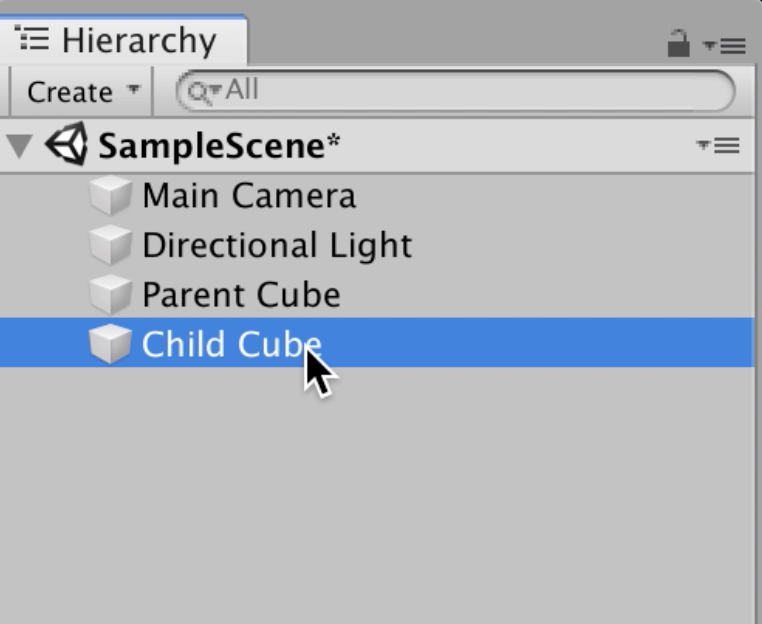
\includegraphics[width=0.25\textwidth]{parent_ui_1}} $\rightarrow$
\raisebox{-.5\height}{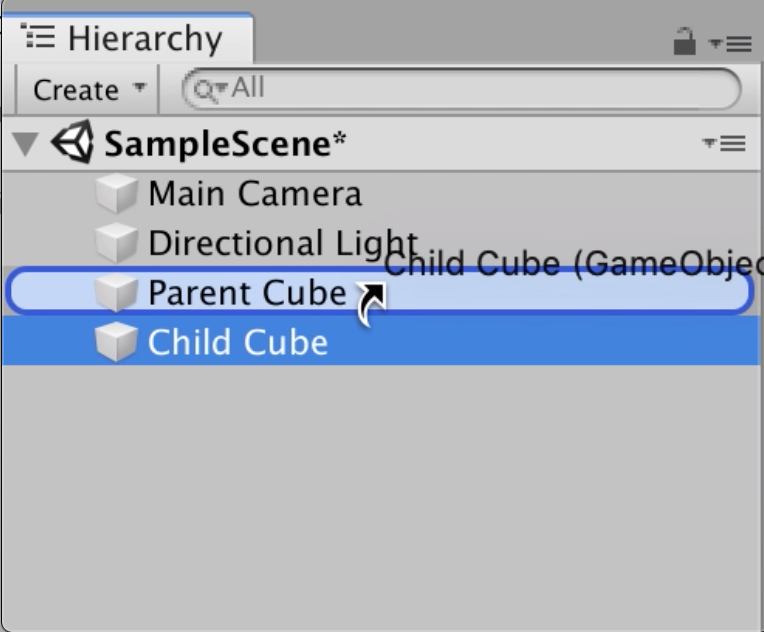
\includegraphics[width=0.25\textwidth]{parent_ui_2}} $\rightarrow$
\raisebox{-.5\height}{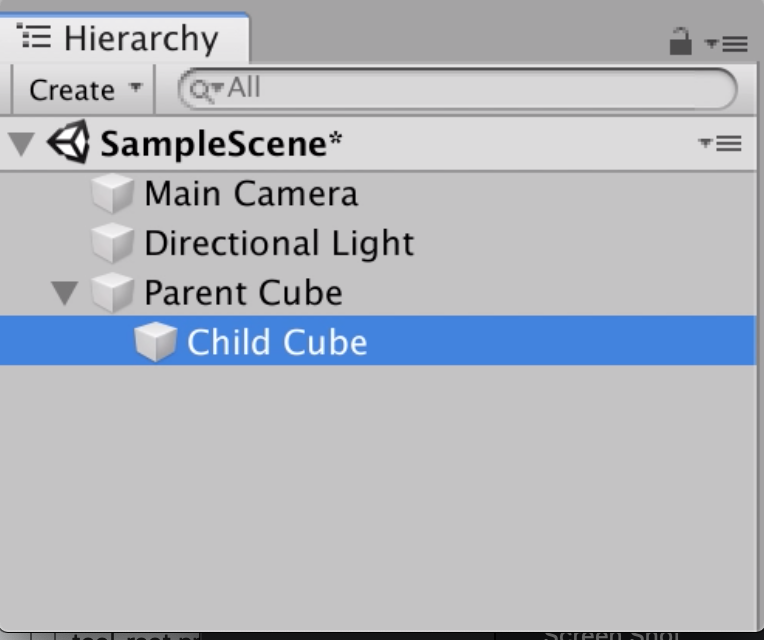
\includegraphics[width=0.25\textwidth]{parent_ui_3}} \\
How to parent two GameObjects in the hierarchy view
\end{center}

After two GameObjects are parented, then manipulating the parent will similarly manipulate the child, as shown below:

\begin{center}
\centering \noindent
\raisebox{-.5\height}{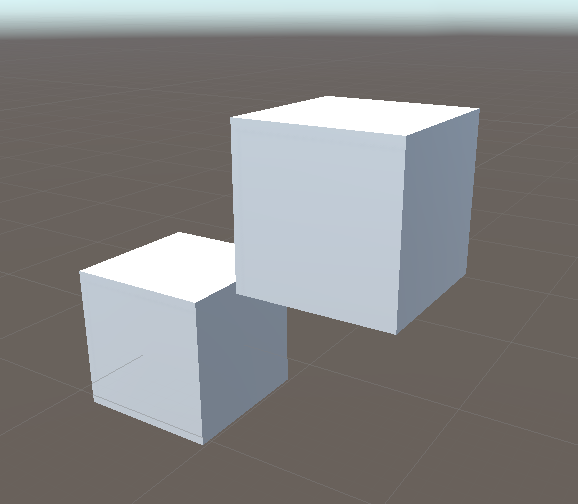
\includegraphics[width=0.25\textwidth]{parent_1}} $\rightarrow$
\raisebox{-.5\height}{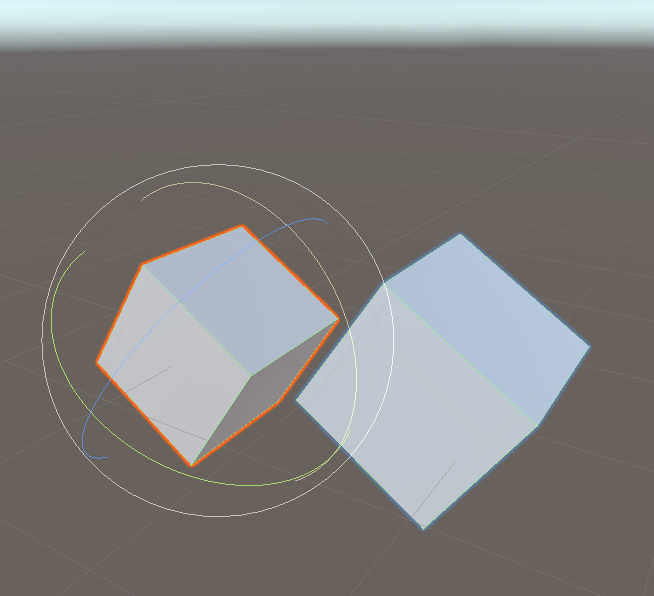
\includegraphics[width=0.25\textwidth]{parent_2}} $\Big/$
\raisebox{-.5\height}{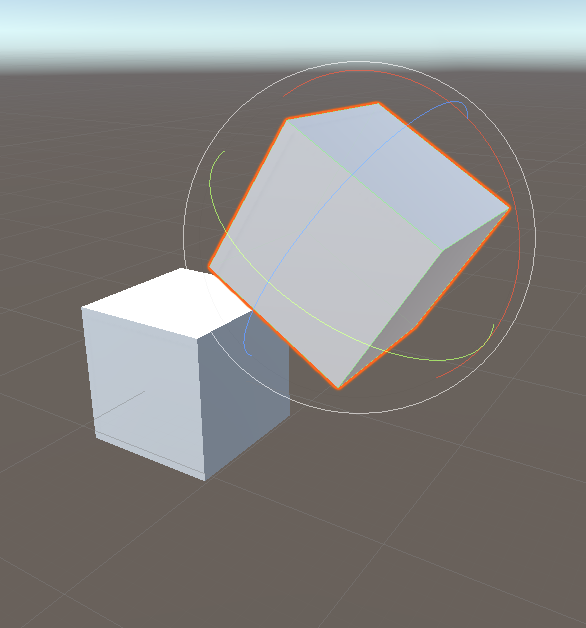
\includegraphics[width=0.25\textwidth]{parent_3}} \\
Left: Without transformation.  Middle: Rotating the parent.  Right: Rotating the child
\end{center}

\section{Composing GameObjects with Components}

\begin{wrapfigure}[13]{r}[50pt]{0.5\textwidth}
    \centering
    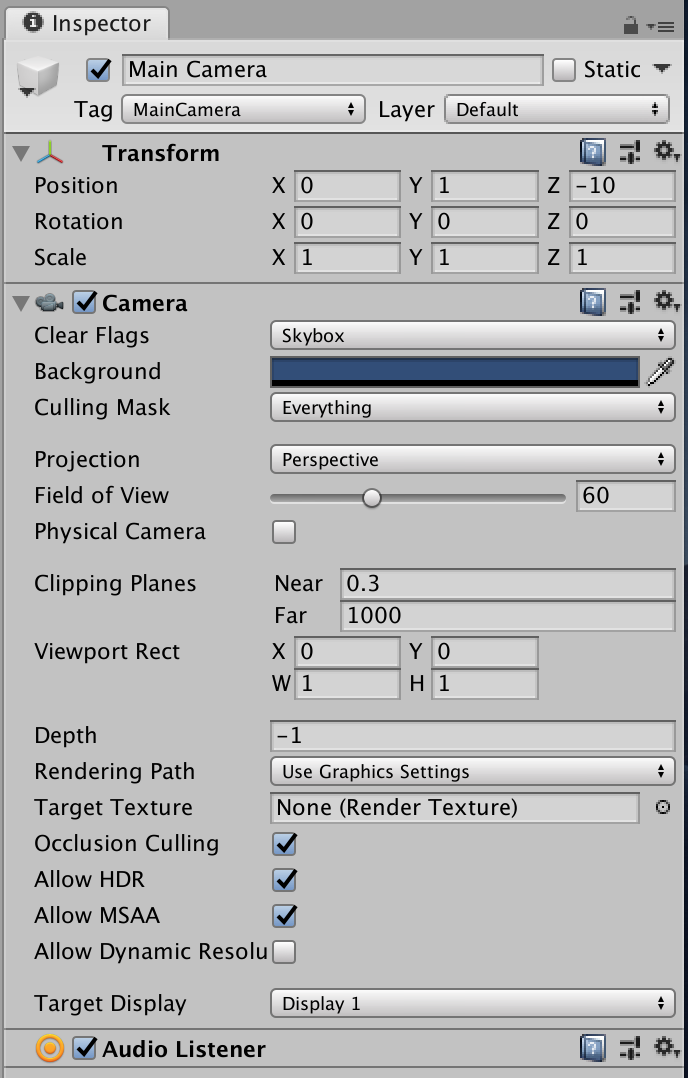
\includegraphics[width=0.25\textwidth]{inspector_camera}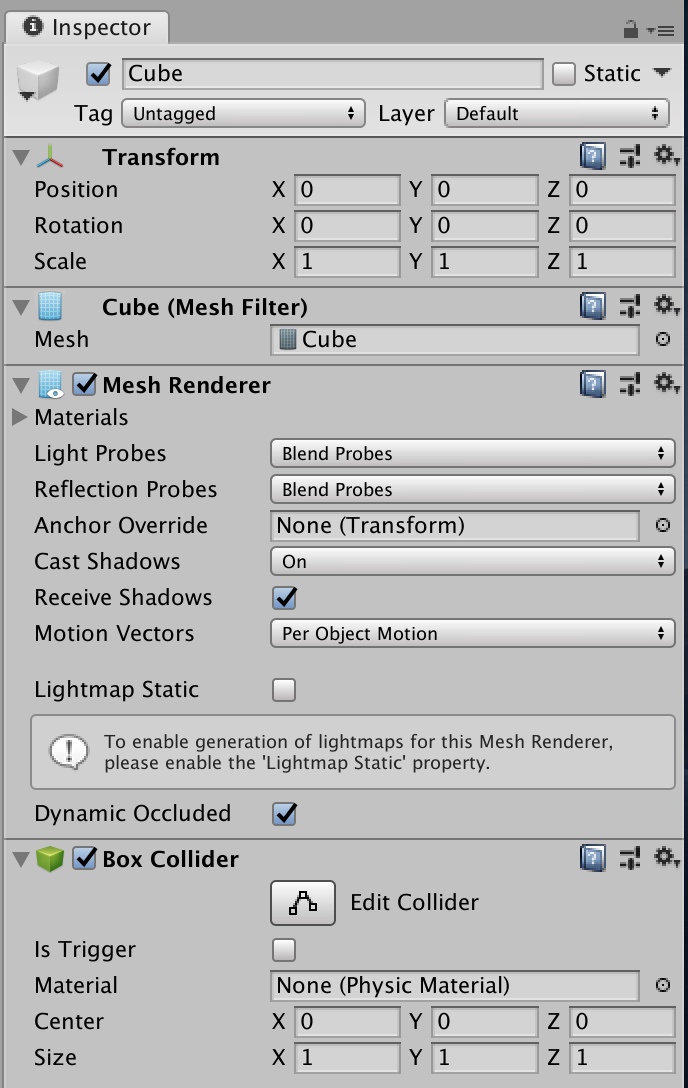
\includegraphics[width=0.25\textwidth]{inspector_cube}
\end{wrapfigure}


You may have noticed by now that as you select GameObjects in the scene, the Inspector panel (on the right) updates depending on the currently-selected GameObject.  Let's take a closer look at the Inspector now.  Select the Cube GameObject that we created earlier.  At the top of the inspector there is a block of \textit{transform attributes} -- these are shared by all GameObjects.  When you use any of the transformation manipulators in the Scene View Tools, these values will change accordingly.  You can also edit these values (for the position, rotation, and scale of the object) in the inspector.  Below the transform attributes there are 3 headings: \textit{Mesh Filter, Mesh Renderer,} and \textit{Box Collider}.

Now click on the \textit{Main Camera} GameObject and take a look at the Inspector.  As mentioned, the transform attributes are still there; you can move and rotate the camera as normal (scaling the camera simply does nothing).  However the Mesh Filter, Mesh Renderer, and Box Collider have been replaced by a two blocks: \textit{Camera} and \textit{Audio Listener}.

These blocks represent the different Components of each GameObject.  A \textbf{Component} is the fundamental building block of GameObjects in Unity -- \textit{all} of the behavior of a GameObject is performed by its components.  For example, the behavior of our cube is encapsulated by its components: the \textit{Mesh Filter} and \textit{Mesh Renderer} define what 3D model should be rendered and how, and the \textit{Box Collider} allows the cube to interact with Unity's physics system.  Similarly, the \textit{Camera} allows one to use a GameObject as a viewport and \textit{Audio Listener} enables 3D positional sound.  Components are also configurable -- try fiddling with the Field of View of the camera for example.

The objects that we have looked at so far were made for us by Unity's interface, however you can build GameObjects "from scratch," by starting with an empty GameObject (an \textbf{Empty GameObject} is one without any components).  Create an empty GameObject via \menu{GameObject > Create Empty} and select it in the hierarchy view.  Now click the \menu{Add Component} button, search for \textit{Mesh Filter}, and hit \keys{Enter}.  You should see a \textit{Mesh Filter} added to your GameObject.  

\begin{center}
\centering \noindent
\raisebox{-.5\height}{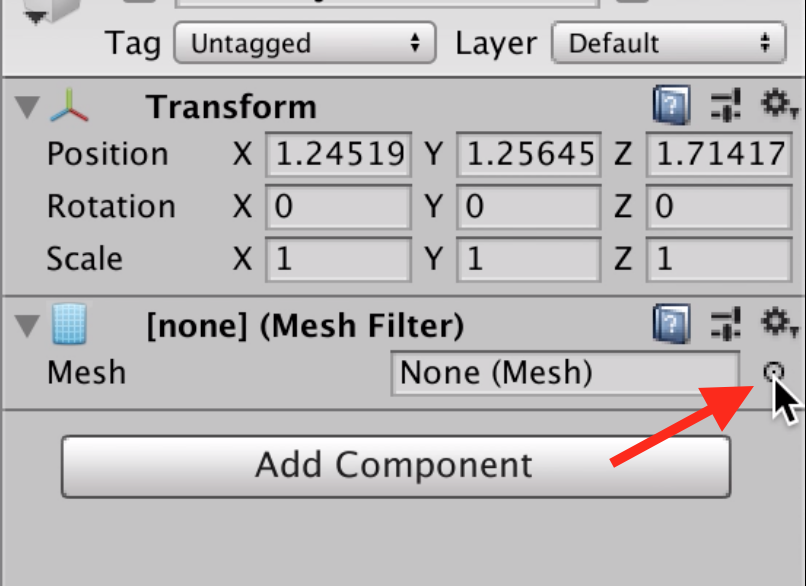
\includegraphics[width=0.25\textwidth]{assign_mesh_1}} $\rightarrow$
\raisebox{-.5\height}{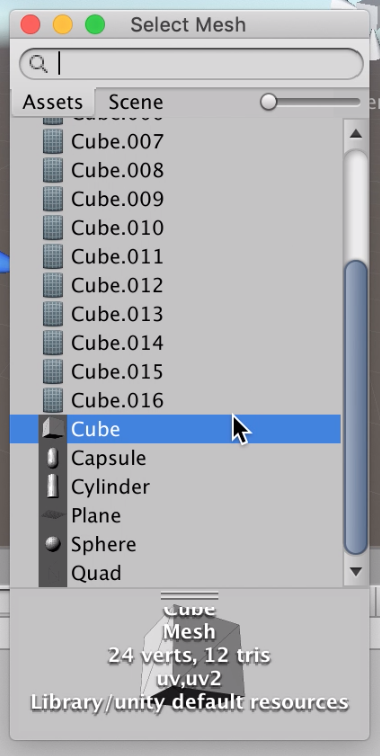
\includegraphics[width=0.15\textwidth]{assign_mesh_2}} $\rightarrow$
\raisebox{-.5\height}{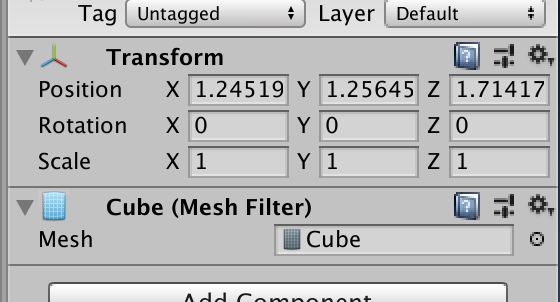
\includegraphics[width=0.25\textwidth]{assign_mesh_3}} \\
Assigning a Mesh to our Mesh Filter
\end{center}

Now try adding the \textit{Mesh Renderer} and \textit{Box Collider} components.  You will notice that the Cube now appears in the scene, but it is an ugly purple color.  This is because we need to add a Material to the cube.  A \textbf{Material} is a special type of Asset that defines how a 3D model should render.  Let's assign the default material to this mesh -- you can do this by expanding the \menu{Materials} menu and assigning the default material as shown below:

\begin{center}
\centering \noindent
\raisebox{-.5\height}{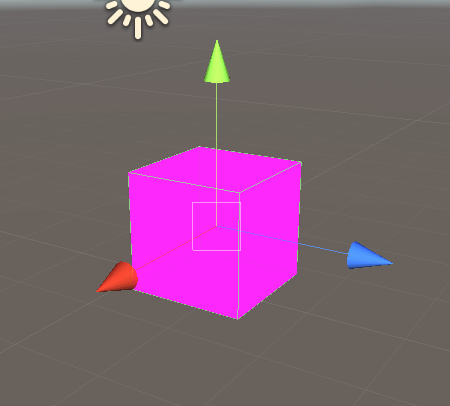
\includegraphics[width=0.20\textwidth]{assign_mat_1}} $\rightarrow$
\raisebox{-.5\height}{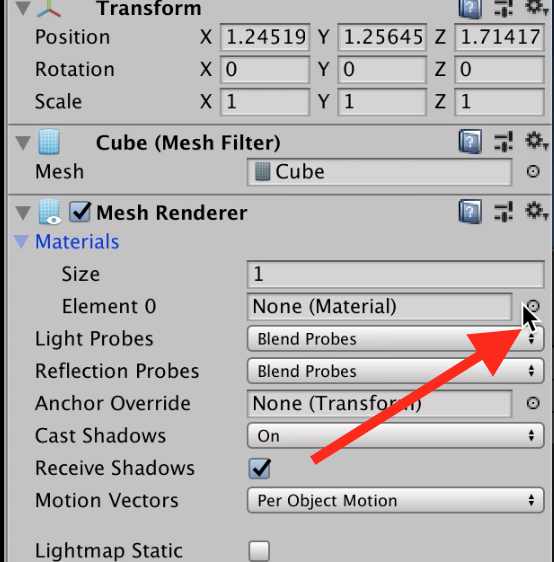
\includegraphics[width=0.25\textwidth]{assign_mat_2}} $\rightarrow$
\raisebox{-.5\height}{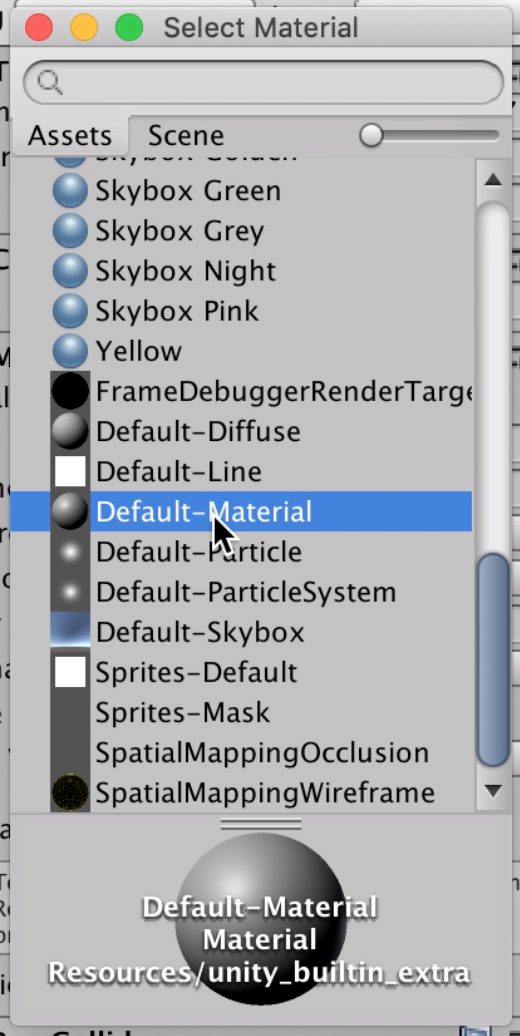
\includegraphics[width=0.15\textwidth]{assign_mat_3}} $\rightarrow$
\raisebox{-.5\height}{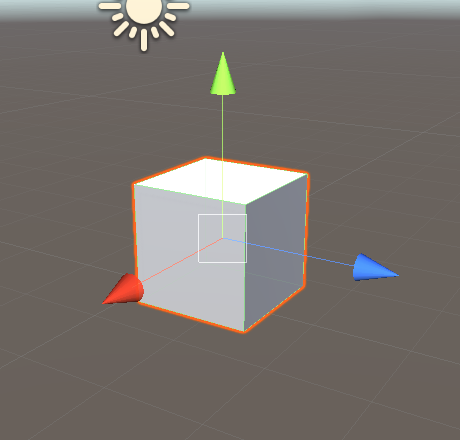
\includegraphics[width=0.20\textwidth]{assign_mat_4}} \\
Assigning a Material to our new GameObject
\end{center}

You can create your own material in the Project view.  Navigate to \menu{Assets > Create > Material}, name the material in the Project view, and tweak the material in the inspector.  Then you can apply the material as before.  Most of the time, we won't need to compose GameObjects manually like this.  However, it is very important to understand that all of Unity's builtin functionality is simply exposed through components!

\section{Importing Asset Packages}

Let's go ahead and import the base assets for this lecture.  You can find the base assets at the link below:
\begin{center}
\href{http://stage.gamecreation.org/StuCo/F19/packages/lec02resources.unitypackage}{http://stage.gamecreation.org/StuCo/F19/packages/lec02resources.unitypackage}
\end{center}

\pagebreak

\begin{wrapfigure}[13]{r}[50pt]{0.5\textwidth}
    \centering
    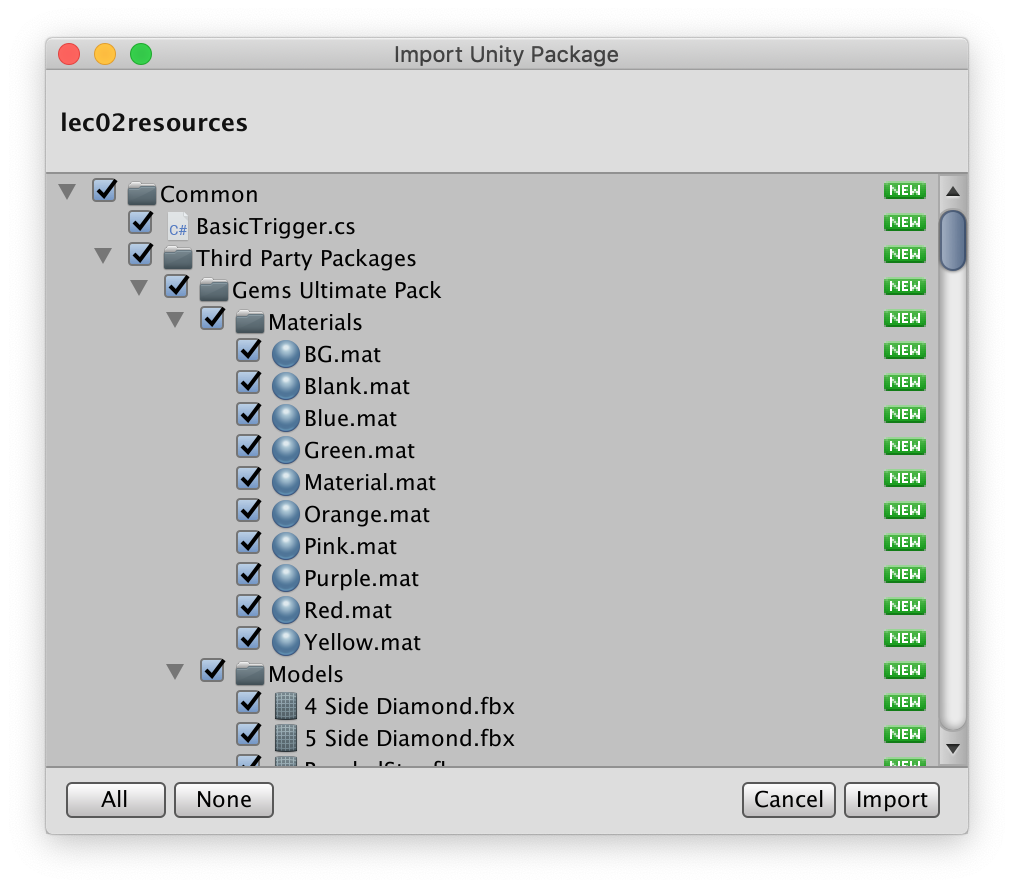
\includegraphics[width=0.5\textwidth]{import-diag}
    Unitypackage Import Dialog
\end{wrapfigure}

This is a .unitypackage file.  Unitypackages are a file format specifically made to import project settings and assets into Unity.  With your new project open, double click on the downloaded file to open it in Unity.  You should see the window to the right.  Click ``All'', then ``Import'' to import the files.

\subsection{Using the Unity Asset Store}

The \textit{Unity Asset Store} is an online store for .unitypackages.  If you don't have access to a larger team, you can use the asset store to get art, scripts, and Editor tools.  In fact, the lecture resources (linked above) contain assets from a few asset store packages (the \href{https://assetstore.unity.com/packages/essentials/asset-packs/standard-assets-32351}{Unity Standard Assets}, a \href{https://assetstore.unity.com/packages/3d/props/3d-crystal-gems-pack-112381}{3D Gem Models pack}, and \href{https://assetstore.unity.com/packages/2d/textures-materials/gridbox-prototype-materials-129127}{some textures for prototyping}).  You'll need a free Unity account to use the Asset Store.

\section{Example Game 1: Plinko}

\begin{center}
\centering \noindent
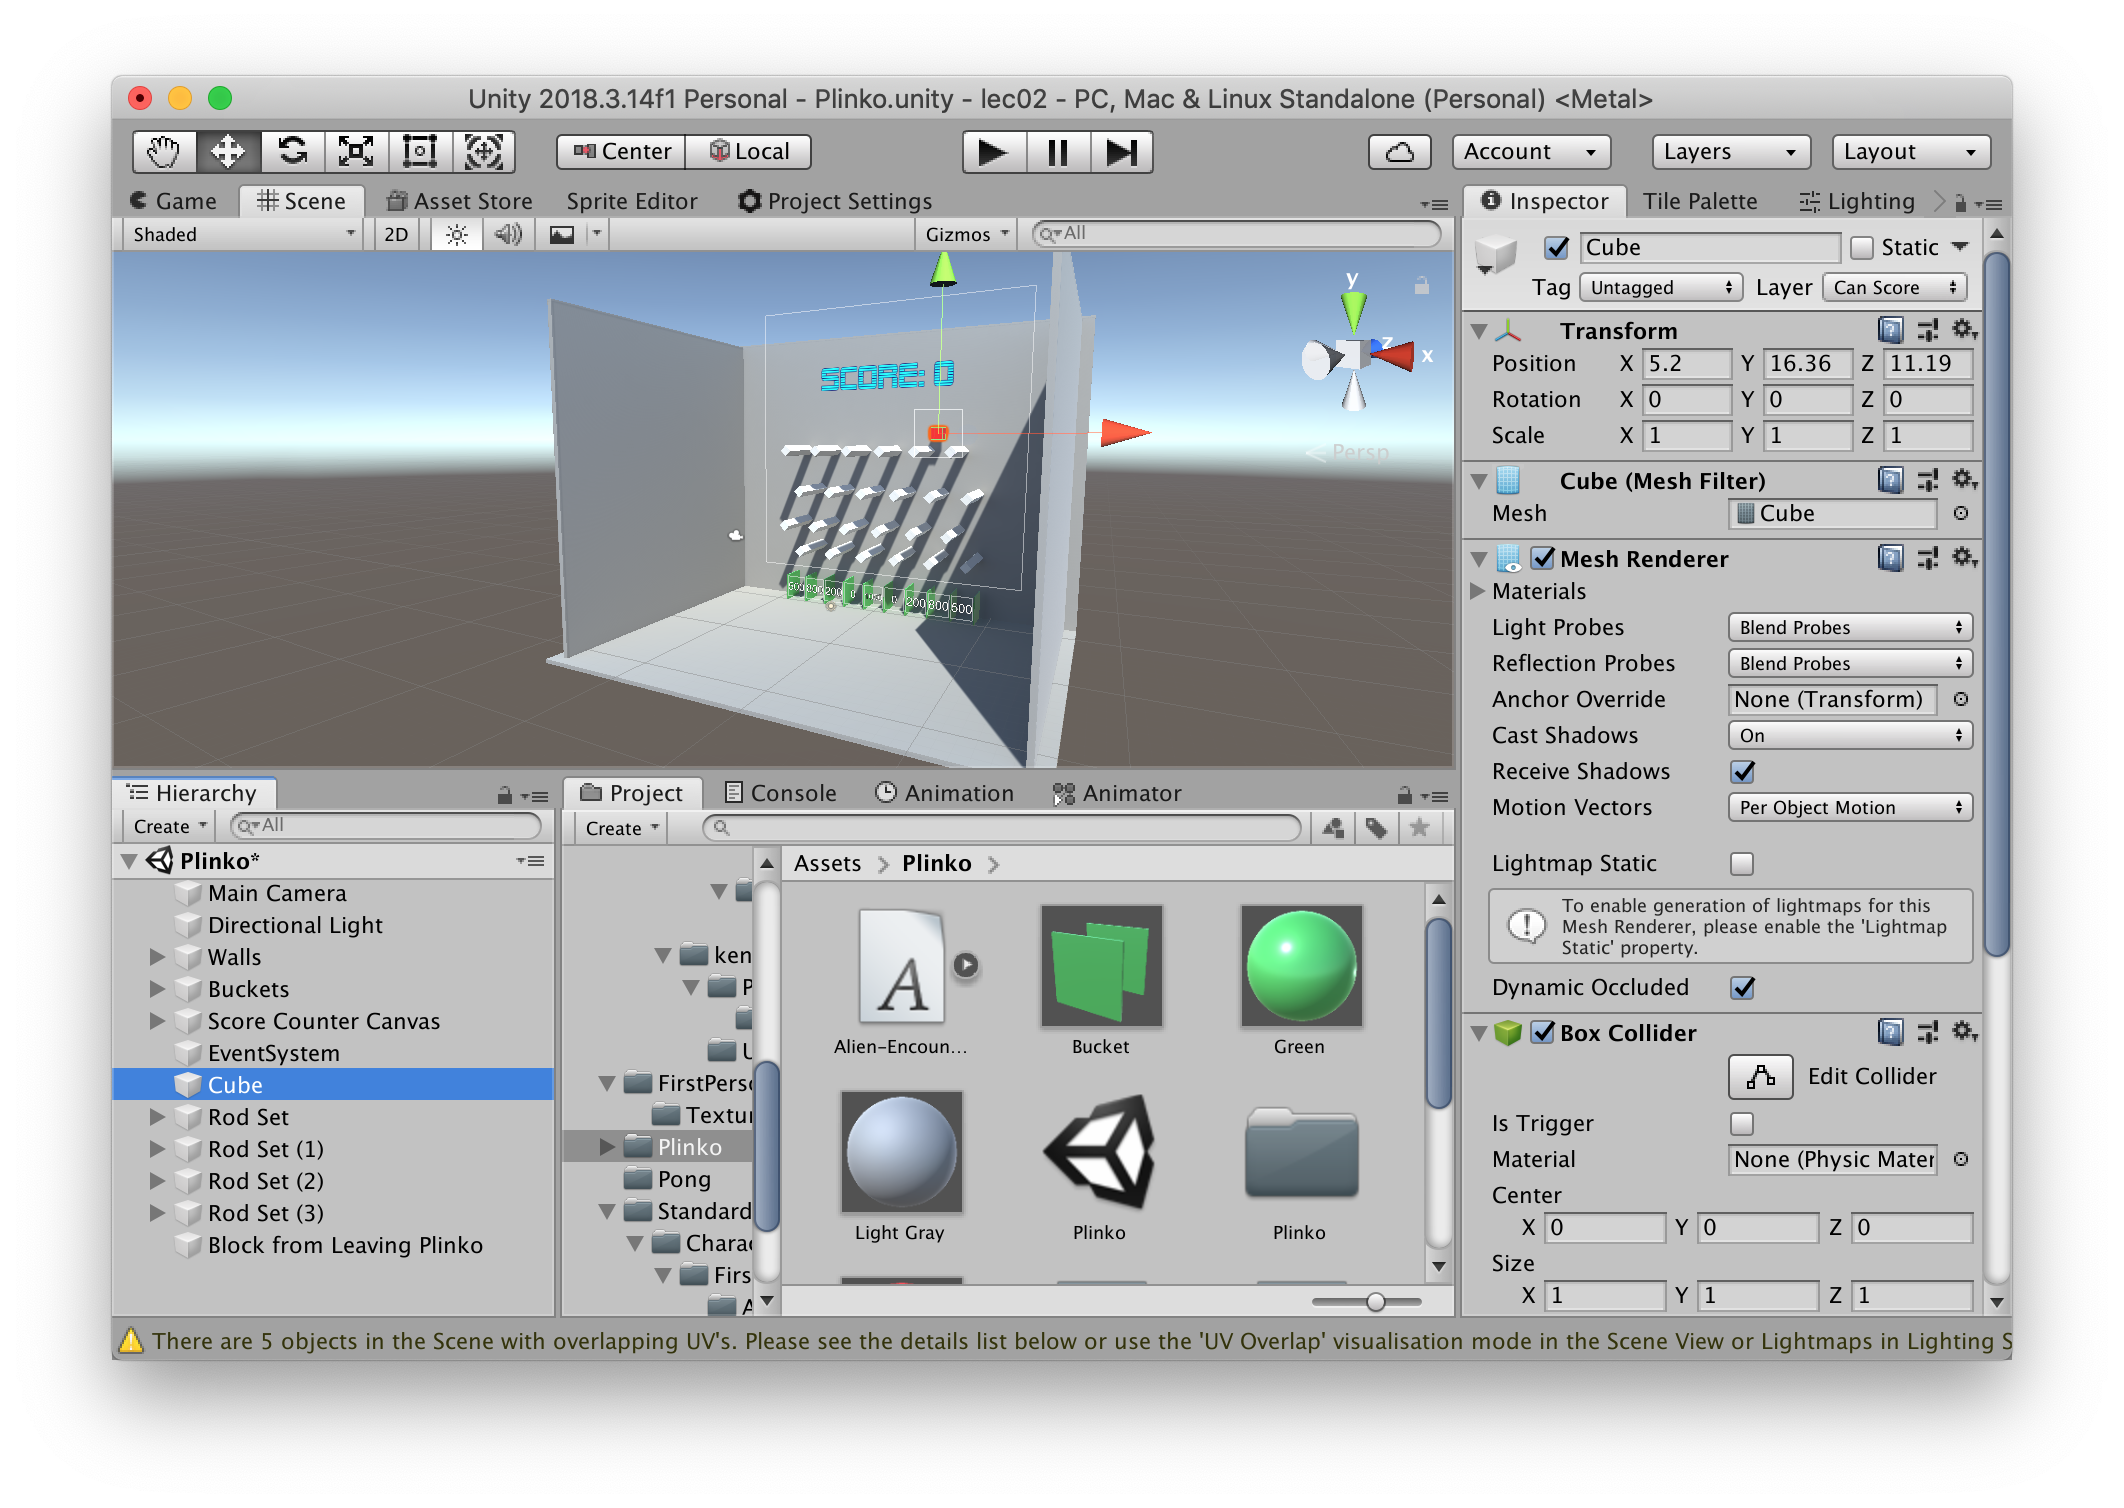
\includegraphics[width=0.85\textwidth]{plinko}
\end{center}

After importing the lecture assets, navigate to \directory{Assets/Plinko/Plinko.scene} in the project view and double click on the scene file to open it.  Press play, and you will see a red cube fall between many pegs into buckets at the bottom of the screen.  When the cube falls in a bucket, the score is incremented.  Try moving the cube around before playing -- notice that it realistically collides with the world and moves in a physically-plausible way, no matter where it starts.

\begin{wrapfigure}{r}[50pt]{0.3\textwidth}
    \centering
    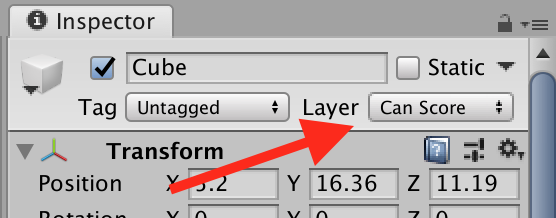
\includegraphics[width=0.3\textwidth]{layers}
    Changing GameObject layers
\end{wrapfigure}
There are two things that are particularly important about the red cube that enable this simple game.  First, the Cube has a Rigidbody component attached.  The \textbf{Rigidbody} component tells Unity to simulate that GameObject via the physics engine.  Unity uses the Collider components attached to the GameObject (or its children) to determine how the object interacts with the world (this cube has a Box Collider attached).  Second, the Cube is marked with a layer called \textit{Can Score}.  All GameObjects belong to a \textbf{Layer} in the scene, and Layers can be used when scripting objects in your game.  In this example, all GameObjects in the \textit{Can Score} layer will increase the score when dropped into a bucket.  All other GameObjects will not be affected.

In the hierarchy view, search for ``Trigger'' and click on one of the GameObjects.  These are the logical GameObjects that help facilitate scoring.  There is a Box Collider here as well, with the ``Is Trigger'' box checked.  ``Is Trigger'' signals to Unity that this collider shouldn't actually be included in physics calculations (that is, nothing should be blocked by it), but it should still receive collision events for scripting purposes.  The other component, called \textit{Basic Trigger}, receives these collision events and passes them on to the scorekeeper script.  The ``Layer Mask'' in \textit{Basic Trigger} is set to \textit{Can Score}, as mentioned.  Importantly, the Basic Trigger component is a \textbf{Custom Script} created specifically for this game.  This is how scripting works in Unity; developers simply create their own custom components!

Now search for the GameObject called ``Score Display Canvas''.  A \textbf{Canvas} component allows you to create UI elements such as text or buttons.  ``Score Display Canvas'' contains a Canvas component (as well as some other Canvas-related supporting components) and a script called \textit{Score Counter}.  The Score Counter script updates the text at the top of the scene.

\section{Example Game 2: Pong}

\begin{center}
\centering \noindent
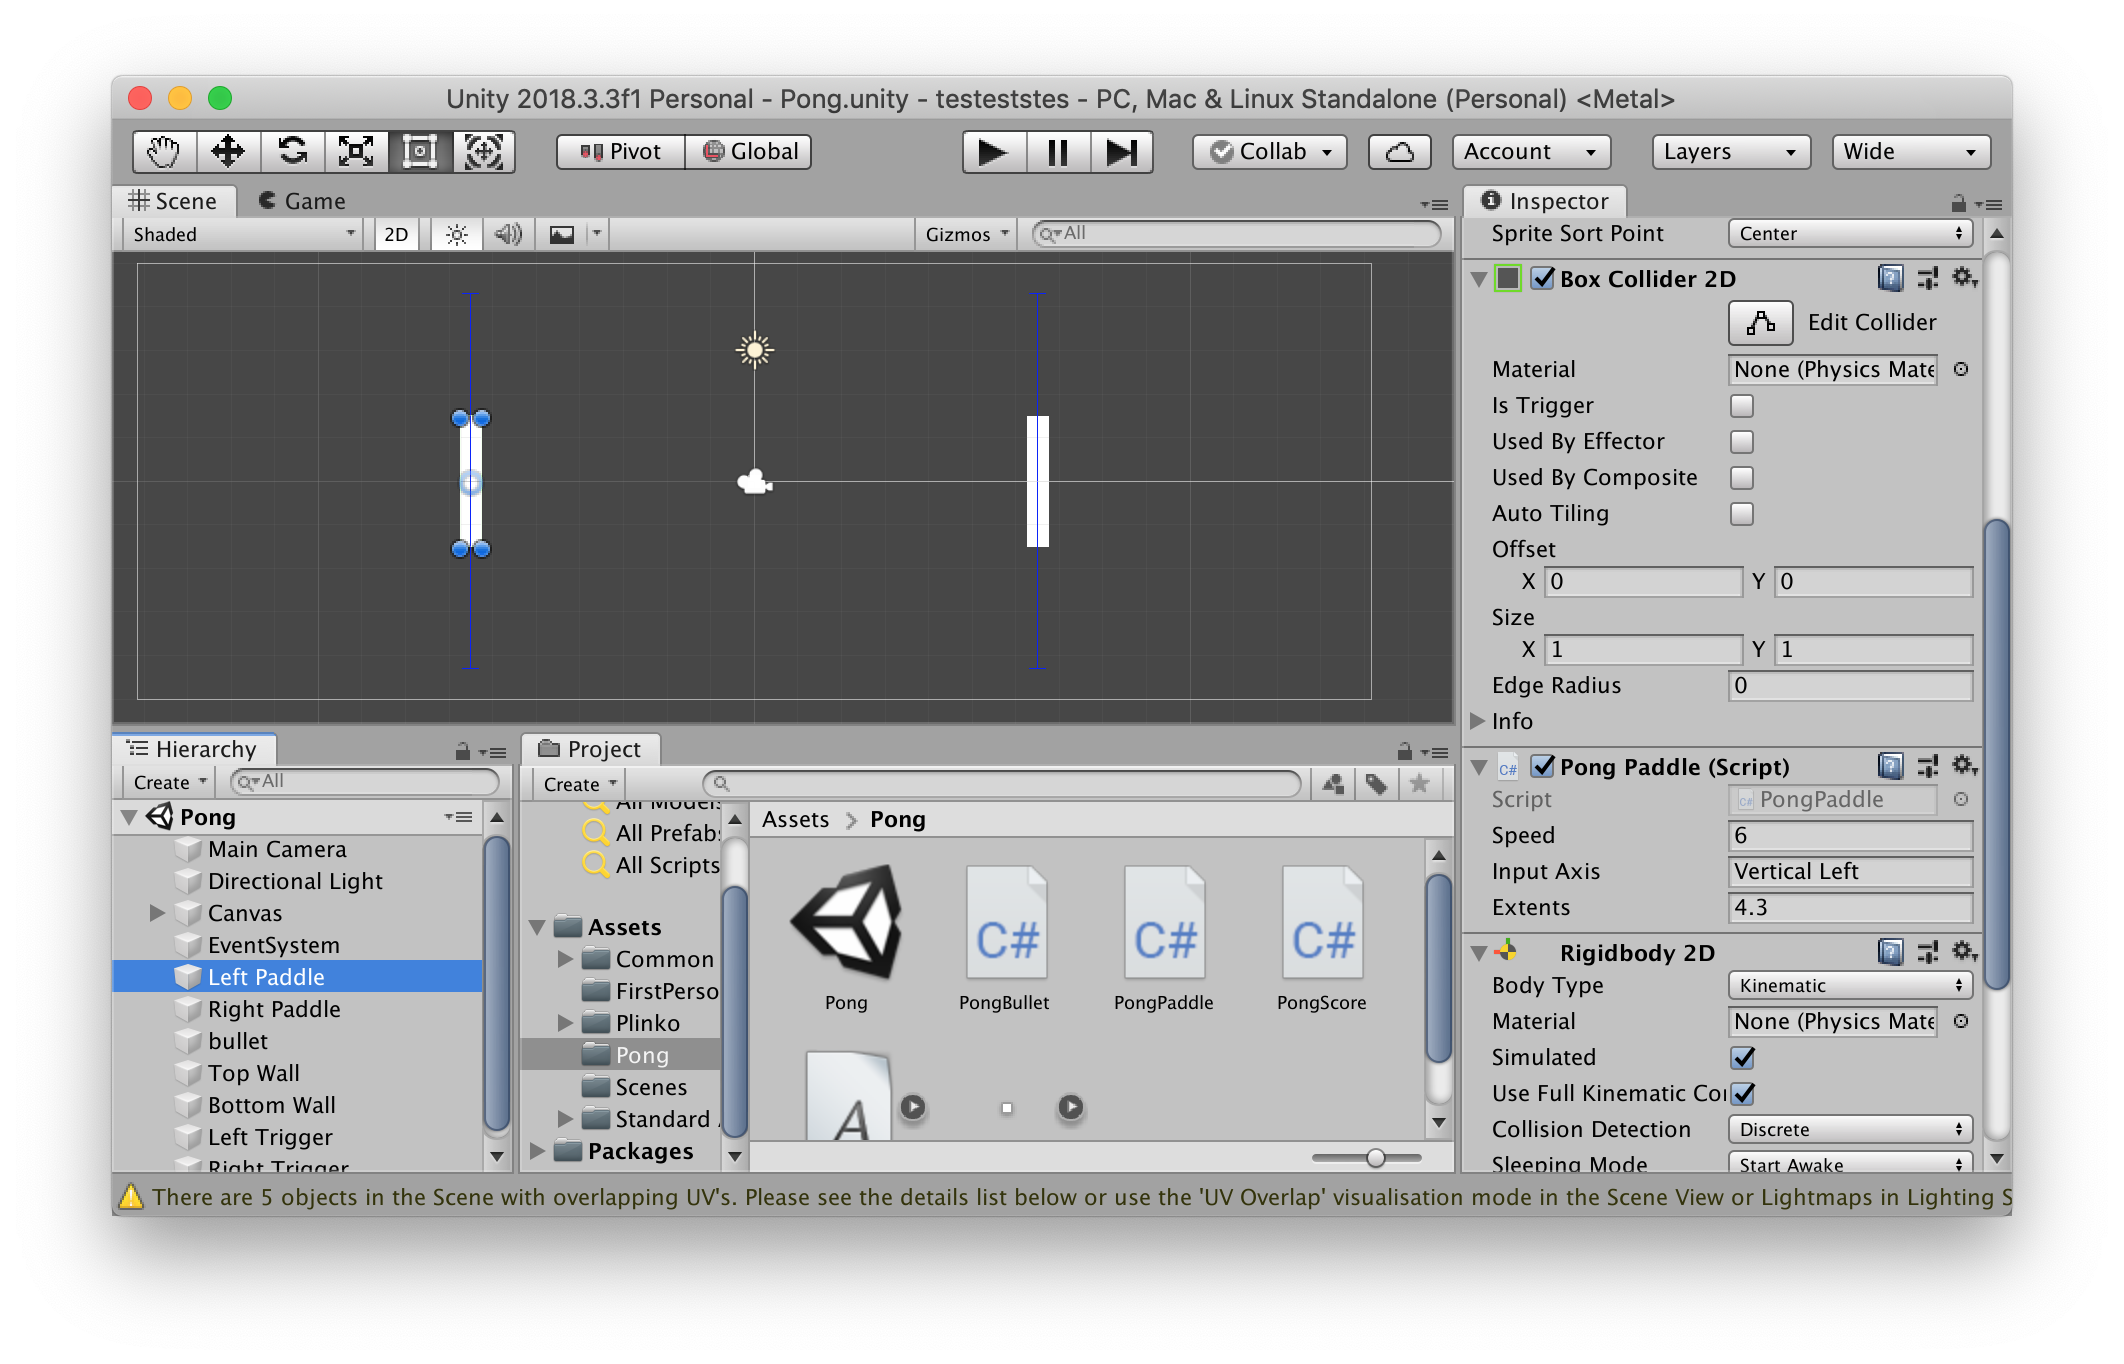
\includegraphics[width=0.85\textwidth]{pong}
\end{center}

The second example scene is classic Pong!  You can try it out by opening the scene at \directory{Assets/Pong/Pong.scene}.  You can control the P1 paddle with the \keys{W} and \keys{S} keys, and the P2 paddle with \keys{\arrowkeyup} and \keys{\arrowkeydown}.  This game is an example of a 2D game in Unity; 2D games in Unity are created in largely the same way as 3D games.  The main difference is that 2D games tend to use 2D-centric components and the camera ignores the Z dimension.  Click the \menu{2D} button at the top of the Scene view to toggle between 2D and 3D editing modes.  It might also be helpful to switch to the Rect Tool 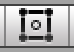
\includegraphics[width=20pt]{tool_rect.png} when working in 2D.

Let's compare the GameObjects in this scene with those in the Plinko example.  As in Plinko, there is a Canvas GameObject that is used to display the score.  A custom component (called \textit{Pong Score}) is attached to the Canvas and handles the score logic.  Now inspect the ``Left Paddle'' GameObject.  The components here are different than with the default 3D cube, but largely similar.  Instead of the Mesh Renderer that is used to render 3D objects, 2D GameObjects use a \textbf{Sprite Renderer} to draw 2D sprites.  Unity actually has two different physics subsystems, one for 2D and one for 3D, so all 2D objects use special 2D physics components.  Instead of a Rigidbody and Box Collider we use a \textbf{Rigidbody 2D} and \textbf{Box Collider 2D}.

The \textit{Pong Paddle} script is used on the ``Paddle Left'' and ``Paddle Right'' GameObjects to facilitate moving the paddles when pressing the corresponding keys.  Try changing the \textit{Speed} attribute to change the movement speed of each paddle.  Similarly the \textit{Pong Bullet} script enables the ball/bullet object to move and bounce correctly off of each paddle and the screen boundaries.

\section{Example Game 3: First Person Game}

\begin{center}
\centering \noindent
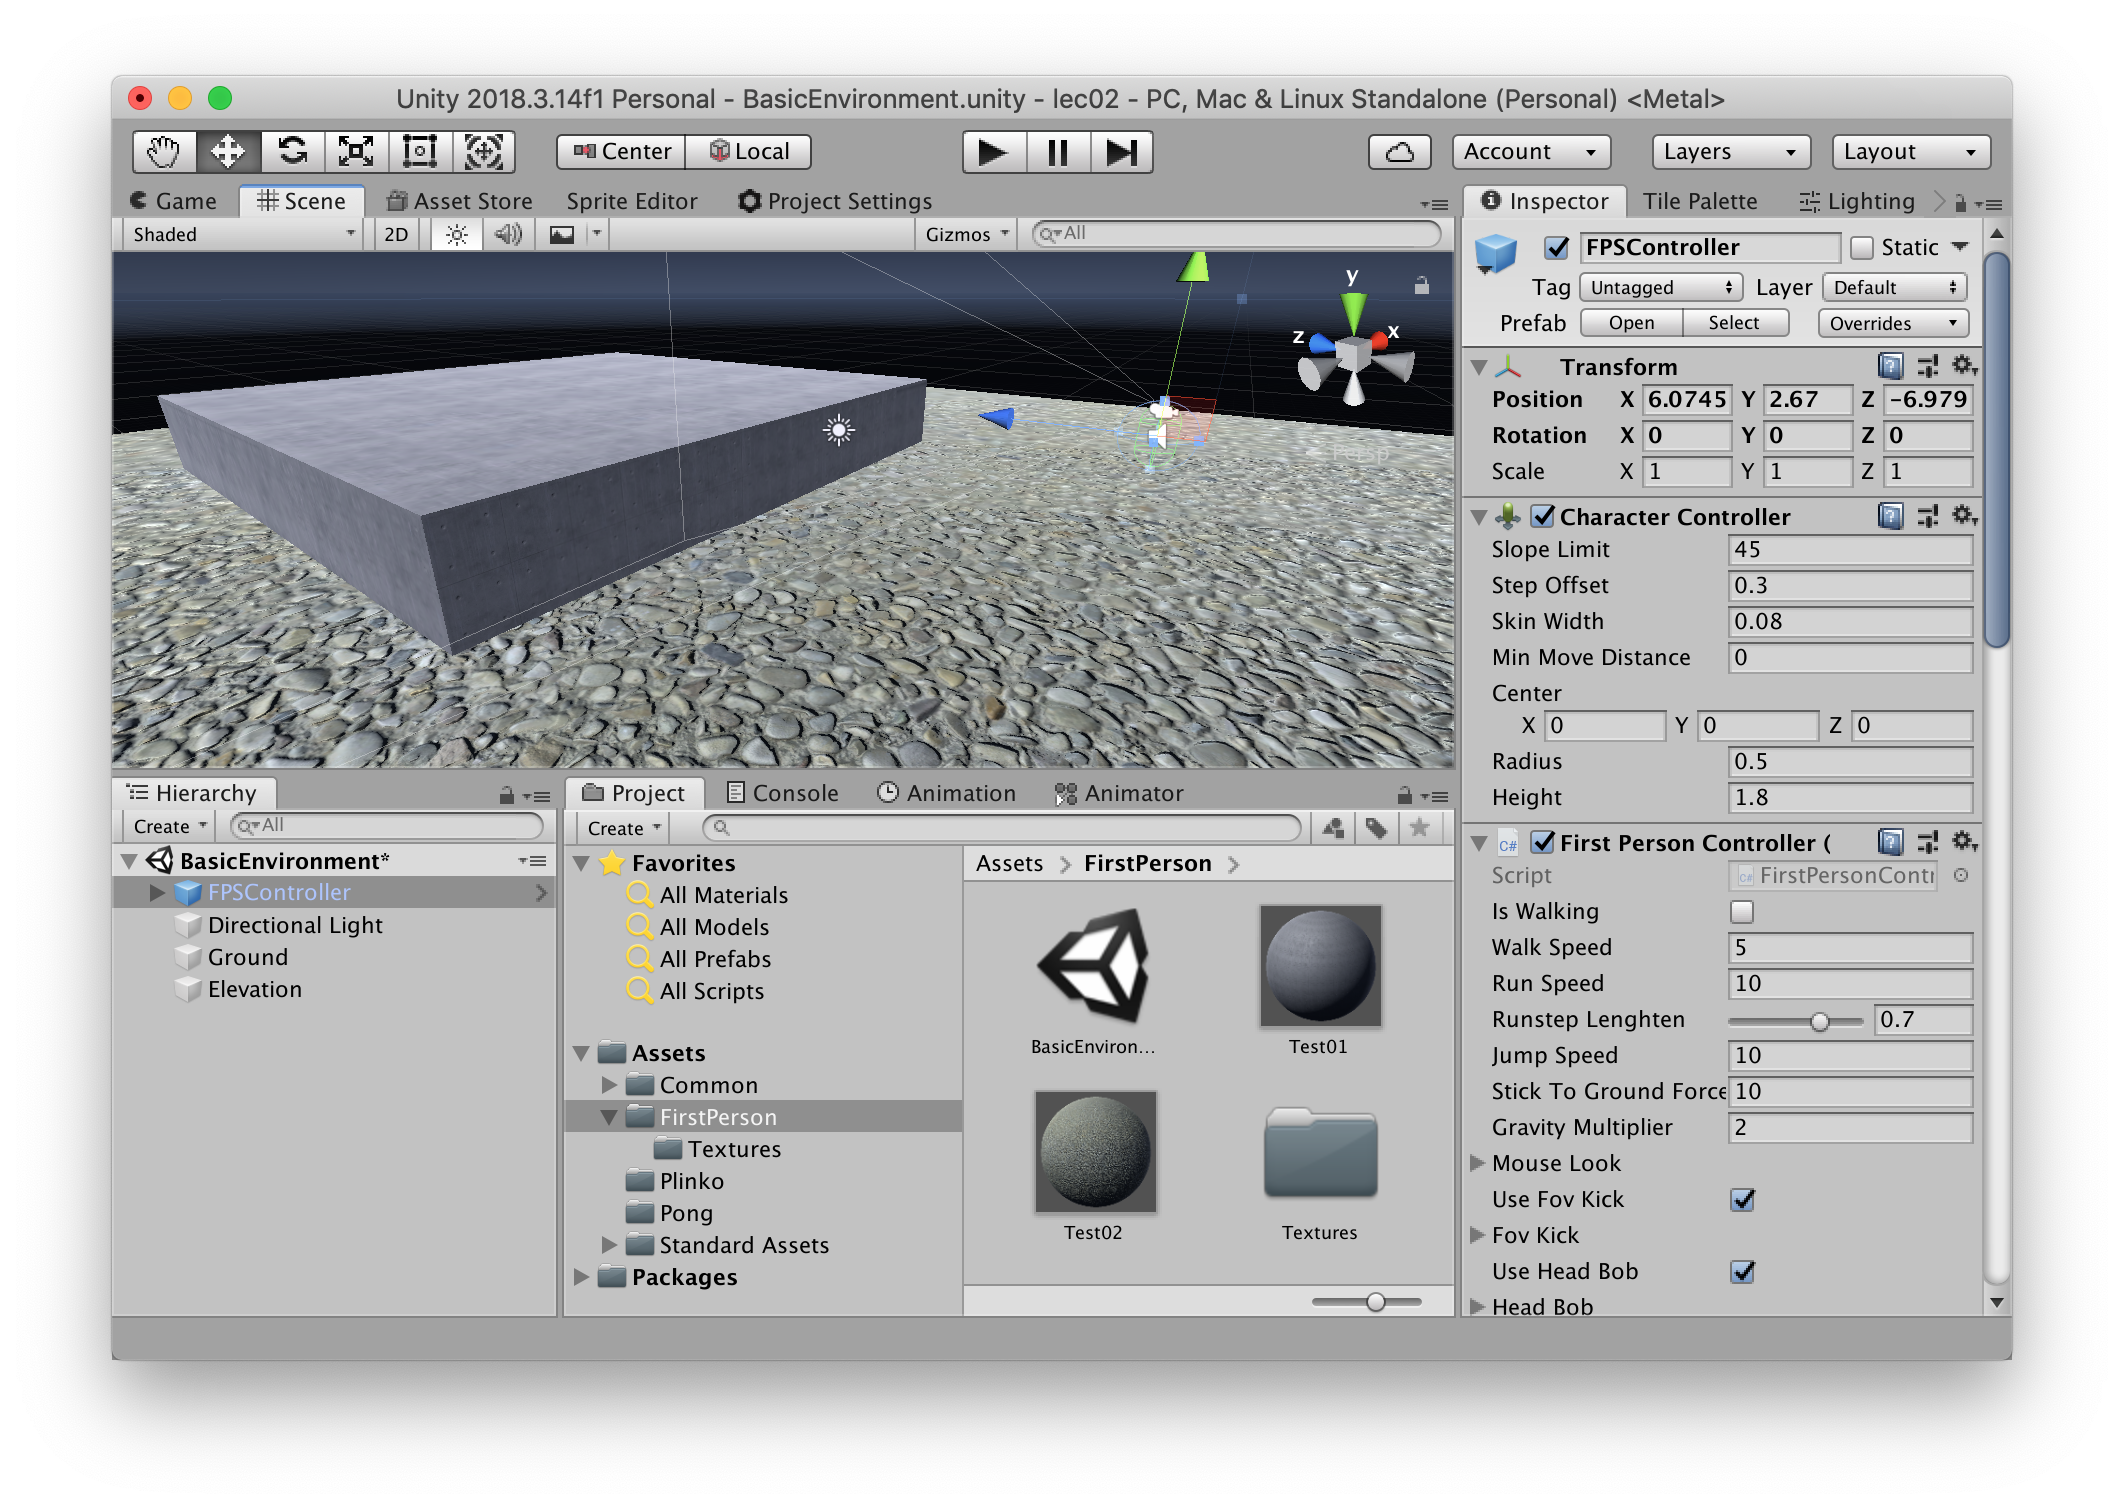
\includegraphics[width=0.85\textwidth]{fpsgame}
\end{center}

The final example isn't a complete game like the previous ones, but it is a good introduction to building expansive environments in Unity.

\subsection{The First Person Controller}

The \textbf{First Person Controller} is part of the Unity Standard Assets and makes it incredibly easy to get a First Person game up and running.  We are using the First Person Controller in this scene - check out the GameObject called ``FPSController''.  The \textbf{Unity Standard Assets} are a package created by Unity that contains a number of often-useful components and assets (you can download them \href{https://assetstore.unity.com/packages/essentials/asset-packs/standard-assets-32351}{here}).  Try changing the parameters of both the \textit{Character Controller} component and the \textit{First Person Controller} component such as Walk/Run speed and height.

To clarify, the \textit{Character Controller} component is built in to Unity and can be used by scripts to move a character GameObject around the scene.  The \textit{First Person Controller} component is a script that comes with the Unity Standard Assets that allows the player to look around with the mouse and move with \keys{W}\keys{S}\keys{A}\keys{D} controls.  The ``FPSController'' GameObject also contains an \textit{Audio Source} component to generate footstep sounds and a \textit{Rigidbody} to receive physics events.

\section{Exercise}

Design one simple modification to any of the three demos that we went over today, and implement it in Unity.  Some ideas include:

\begin{itemize}
    \item Modifying Plinko by adding more obstacles, so that it is harder to score well
    \item Modifying Pong so that the ball's behavior is more complex (it is necessary to be familiar with C\# scripting first to do this)
    \item Creating a more complex environment in the First Person scene
\end{itemize}

\end{document}